\documentclass{article}
\usepackage{amsmath}
\usepackage{amssymb}
\usepackage{algorithm}
\usepackage{float}
\usepackage{color}
\usepackage{multicol}
\usepackage{forloop}
\usepackage{graphicx}
\usepackage[margin=0.8in]{geometry}
\usepackage{caption}
\usepackage{enumerate}
\graphicspath{ {.} }
\title{STAT 2509B4 \\
	\large{Assignment 1}}
\author{Krystian Wojcicki, 101001444}
\date{Winter 2020}

\begin{document}
\maketitle

\begin{enumerate}[1.]
\item

\textbf{Define the following:}
\begin{enumerate}[(i)]
  \item \textbf{variable: } a characteristic that varies from a person or a thing to another one, or over time.
  \item \textbf{experimental unit: } indiviudals or objects on which a variable is measured
  \item \textbf{a single measurement: } a single measurement is the value of a variable measured on a an experimental unit.
  \item \textbf{population: } the set of all measurements of a variable of interest to the investigator
  \item \textbf{sample: } a subset of measurements selected and observed from the population of interest

\end{enumerate}

\item
\begin{enumerate}[(a)]
\item
\textbf{List the possible types of variables:} The possible types of variables are qualitative and quantitative. Qualitative can be split up into pure qualitative and qualitative ranked. Quantitative can be split up into quantitative \& discrete and quantitative \& continuous.

\item
\textbf{Identify the following variables as either “pure qualitative” (or “pure categorical”),“qualitative \& ranked” (or “categorical \& ranked)”, “quantitative \& discrete”, or “quantitative \& continuous”:}
\begin{enumerate}[(i)]
  \item \textbf{Time until a bulb burns out: } quantitative \& continuous
  \item \textbf{Beer tasting ranking (excellent, good, fair, or poor): } qualitative \& ranked
  \item \textbf{Student ID number: } pure qualitative
  \item \textbf{Number of cars entering Carleton each day: } quantitative \& discrete
  \item \textbf{Average daily temperature in Ottawa during January: } quantitative \& continuous
  \item \textbf{Letter grade of a course (A, B, C, D, E, or F): } qualitative \& ranked
  \item \textbf{Number of M\&M candies in a bag: } quantitative \& discrete
  \item \textbf{Blood type of a person: } pure qualitative
\end{enumerate}
\end{enumerate}

\item
\textbf{Consider a normal population distribution with the value of the standard deviation $\sigma$ known}
\begin{enumerate}[(a)]
\item
\textbf{What are the confidence level for the following confidence intervals about the population mean:}
\begin{enumerate}[(i)]
  \item \textbf{$\bar{x} \pm 1.96\sigma/\sqrt{n}$: } 95\%
  \item \textbf{$\bar{x} \pm 2.65\sigma/\sqrt{n}$: } 99.2\%
  \item \textbf{$\bar{x} \pm 3.34\sigma/\sqrt{n}$: } N/A as value not present in the given z table.
\end{enumerate}

\item
\textbf{What value of $z$ in the confidence interval formula }
\begin{gather*}
(\bar{x} - z_{\alpha/2}\sigma/\sqrt{n}, \bar{x} + z_{\alpha/2}\sigma/\sqrt{n} )
\end{gather*}
\textbf{results in a confidence level of}

\begin{enumerate}[(i)]
  \item \textbf{97.96\%: } $\to 1 - \alpha = 0.9796 \to \alpha = 0.0204 \to \alpha / 2 = 0.0102 \to z_{\alpha/2} =  2.32$
  \item \textbf{78.88\%: } $\to 1 - \alpha = 0.7888 \to \alpha = 0.2112 \to \alpha / 2 = 0.1056 \to z_{\alpha/2} = 1.25$
  \item \textbf{99.94\%: } $\to 1 - \alpha = 0.9994 \to \alpha = 0.0006 \to \alpha / 2 = 0.0003 \to z_{\alpha/2} = $ N/A as value not present in given z table.
\end{enumerate}
\end{enumerate}

\item
\textbf{Which of the following histograms looks like a histogram for data from a normal distribution? \underline{Explain}}
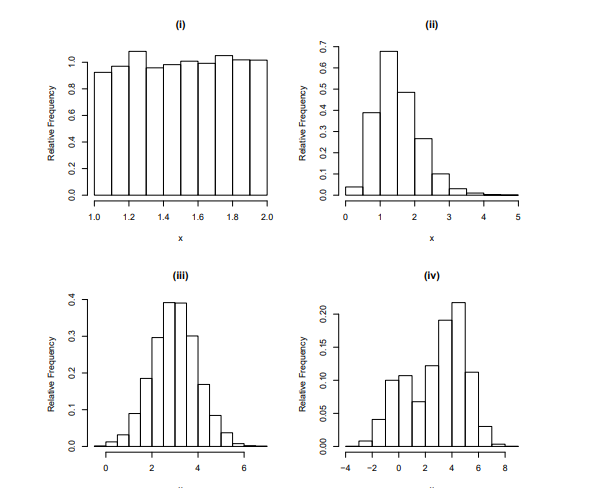
\includegraphics{graphs}

Graph \#3 looks like a histogram displaying a normal distribution. This is because a normal distribution is characterized by a symmetric, bell-shaped curve. All the other graphs are either non-symmetric or not bell shaped. 

\item
\textbf{Let $X$ be a random variable having a normal distribution with mean $\mu$ and standard deviation $\sigma$. Let $c$ be a constant.}
\textbf{Find the \underline{distribution}, \underline{mean} and \underline{standard deviation} of each of the following random variables:}
\begin{enumerate}[(i)]
  \item \textbf{$X + c$: } as taught in class if $X$ is a random variable with a normal distribution then $X \sim N(\mu, \sigma^2)$. Meaning $X + c$ (where $c$ is a constant) gives us $X + c \sim N(\mu + c, \sigma^2)$. Therefore for $X + c$ is a normal distribution, with a mean of $\mu + c$ and standard deviation of $\sigma$. 
  \item \textbf{$(X - \mu)/\sigma$: } as $X \sim N(\mu, \sigma^2)$ then $z := (X - \mu)/\sigma \sim N(0, 1)$. Meaning $(X - \mu)/\sigma$ is a standard normal distribution, with a mean of 0 and standard deviation of 1.
\end{enumerate}

\item
\textbf{Find the following values from the upper-tail z and t tables:}
\begin{enumerate}[(i)]
  \item \textbf{$z_{0.0154}$ = } 2.16
  \item \textbf{$z_{0.9846}$ = } $z_{0.0154} = 2.16$
  \item \textbf{$z_{0.1215}$ = } 1.17
  \item \textbf{$t_{6;0.05}$ = } 1.943
  \item \textbf{$-t_{10;0.025}$ = } -2.228
  \item \textbf{$t_{10;0.975}$ = } $-t_{10;0.025} = -2.228$ 
\end{enumerate}

\item
\begin{enumerate}[a]
  \item \textbf{Define two-sided and one-sided hypotheses about a parameter $\theta$ and give the steps involved in their testing: }
\\
2-sided hypothesis is a 2 tailed test for testing parameter $\theta \neq 0$. For example $H_0 : \theta = 0$ or $H_a : \theta \neq 0$.
\\
1-sided hypothesis is a 1 tailed test for testing parameter $\theta < 0$ or $\theta > 0$. For example $H_0 : \theta \leq 0$ vs $H_a: \theta > 0$ or the other side, $H_0 : \theta \geq 0$ vs $H_a : \theta < 0$.
\\
The steps involved for either hypothesis is as follows:
\begin{enumerate}[1)]
  \item State $H_0$ and $H_a$
  \item Find the test statistic for the test
  \item Find the rejection or critical region (or p-value)
  \item Draw conclusion
\end{enumerate}

  \item \textbf{For any hypothesis test, what are the two types of errors that may be made? Explain.}
\\
Type I error is an  error when we reject $H_0$ when it is in fact true. The probabiltiy of type I error is $\alpha$.
\\
Type II error is an error when we do not reject $H_0$ when it is in fact false. The probability of type II error is $\beta$.
\end{enumerate}

\item
\textbf{Classify each of the following quantities as either a parameter or a statistic:}
\begin{enumerate}[(i)]
  \item \textbf{$\sigma^2$: } parameter
  \item \textbf{$\hat{\beta}_1$: } statistic
  \item \textbf{$s^2$: } statistics
  \item \textbf{$\mu$: } parameter
  \item \textbf{$\beta_0$: } parameter
  \item \textbf{$\bar{x}$: } statistic
\end{enumerate}

\item
\textbf{Show that:} \\
$S_{xy} = \sum_{i=1}^{n}(x_i - \bar{x})(y_i - \bar{y}) = \sum_{i=1}^{n}x_iy_i - \frac{(\sum_{i=1}^{n}x_i)(\sum_{i=1}^{n}y_i)}{n}$

\begin{gather*}
\sum_{i=1}^{n}(x_i - \bar{x})(y_i - \bar{y}) \\
= \sum_{i = 1}^{n}(x_iy_i - x_i\bar{y} - \bar{x}y_i + \bar{x}\bar{y}) \\
= \sum_{i = 1}^{n}(x_iy_i - x_i\bar{y} - \bar{x}y_i) + n\bar{x}\bar{y} \\
= \sum_{i = 1}^{n}(x_iy_i) - \bar{y}\sum_{i=1}^{n}x_i - \bar{x}\sum_{i=1}^{n}y_i + n\bar{x}\bar{y} \\
= \sum_{i = 1}^{n}(x_iy_i) - \bar{y}\bar{x}n - \bar{x}\bar{y}n + n\bar{x}\bar{y} \\
= \sum_{i = 1}^{n}(x_iy_i) - 2\bar{y}\bar{x}n + n\bar{x}\bar{y} \\
= \sum_{i = 1}^{n}(x_iy_i) - \bar{y}\bar{x}n \\
= \sum_{i = 1}^{n}(x_iy_i) - \frac{\sum_{i=1}^{n}y_i}{n}\frac{\sum_{i=1}^{n}x_i}{n}n \\
= \sum_{i=1}^{n}x_iy_i - \frac{(\sum_{i=1}^{n}x_i)(\sum_{i=1}^{n}y_i)}{n}
\end{gather*}

Therefore $\sum_{i=1}^{n}(x_i - \bar{x})(y_i - \bar{y}) = \sum_{i=1}^{n}x_iy_i - \frac{(\sum_{i=1}^{n}x_i)(\sum_{i=1}^{n}y_i)}{n}$

\end{enumerate}
\end{document}